%
% kehrwert-symmetrisch.tex
%
% (c) 2026 Damien Flury, OST Ostschweizer Fachhochschule
%
\begin{figure}
\centering
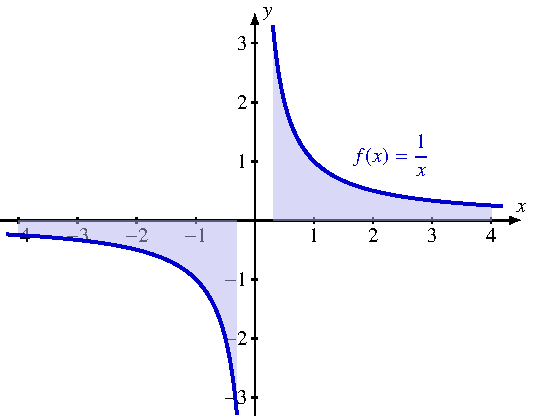
\includegraphics{papers/hauptwert/images/kehrwert-symmetrisch.pdf}
\caption{Graph der Funktion $f(x)=1/x$ mit Polstelle bei $x=0$.
Die schraffierten Flächen zeigen die symmetrische Wahl der
Integrationsgrenzen $\pm\epsilon$ und $\pm R$ um die Polstelle.
\label{hauptwert:figure:kehrwert-symmetrisch}}
\end{figure}
